\documentclass{beamer}
\usetheme{Madrid}
\usepackage{pgfplots}
\pgfplotsset{compat=1.15}
\usepackage{mathrsfs}
\usetikzlibrary{arrows}
\usepackage[utf8]{inputenc}
\usepackage{xcolor}
\usepackage{hyperref}
\usepackage{fancyvrb}
\usepackage{comment}
\usepackage{listings}
\usepackage{color}
\definecolor{munsell}{rgb}{0.0, 0.5, 0.69}
\definecolor{dkgreen}{rgb}{0,0.6,0}
\definecolor{gray}{rgb}{0.5,0.5,0.5}
\definecolor{mauve}{rgb}{0.58,0,0.82}
\definecolor{minas}{RGB}{0.244, 0.172, 0.36}
\definecolor{PUJ}{RGB}{44, 86, 151}
\definecolor{PUJ2}{RGB}{43, 93, 156}
\definecolor{PUJ3}{RGB}{20, 52, 107}
\definecolor{cyandk}{rgb}{0.0, 0.72, 0.92}
\setbeamerfont{frametitle}{size=\LARGE ,series=\bfseries}
\setbeamercolor{frametitle}{fg=PUJ2, bg=white} %% title of the beamer
\setbeamercolor{titlelike}
{parent=structure,bg=PUJ2}
\setbeamercolor{title}{fg=white, bg=PUJ3} 
%\setbeamercolor{navigation symbols}{fg=white, bg=white}
\setbeamercolor*{palette primary}{use=structure,fg=black,bg=yellow}
\setbeamercolor*{palette secondary}{use=structure,fg=white,bg=PUJ3}
\setbeamercolor*{palette tertiary}{use=structure,fg=white,bg=PUJ3}


%% code information
\lstset{frame=tb,
  language=Python,
  aboveskip=3mm,
  belowskip=3mm,
  showstringspaces=false,
  columns=flexible,
  basicstyle={\small\ttfamily},
  numbers=none,
  classoffset=1,
  morekeywords={True,False}, keywordstyle=\color{munsell}, 
  classoffset=0, 
  keywordstyle=\color{blue},  
  commentstyle=\color{dkgreen},
  stringstyle=\color{PUJ3},
  numberstyle=\tiny\color{gray},
  breaklines=true,
  breakatwhitespace=true,
  tabsize=4,
}

%% You can change default language in the middle of document with \lstset{language=Java}.


%% PUT or Remove the logo in a slide.


%% Information topic

\institute{Javeriana}
\date{2020}

\title[Pontificia Universidad Javeriana] %optional
{ Introduction a first course in Programming to Data Science}
\subtitle{Using python.}

\author[Iván Andrés Trujillo Abella] 
{Iván Andrés Trujilllo Abella}

\institute[] 
{
  Facultad de Ingenieria\\
  Pontificia Universidad Javeriana
  \and
  
\textbf{ trujilloiv@javeriana.edu.co}
}

\date[MITA] % (optional)

\newif\ifplacelogo % create a new conditional
\placelogotrue % set it to true
%\logo{\ifplacelogo\color{red}\rule{.5cm}{.5cm}\fi}
\logo{\ifplacelogo 
\includegraphics[height= 2.0cm]{pujshield.eps}\fi}

\begin{document}




\frame{\titlepage}




\begin{frame}{What is involved in programming}

\begin{itemize}
\item creativity 
\item abstraction
\item divisibility 
\end{itemize}

\end{frame}



\begin{frame}{Algorithmic thinking}
This is more important that a concrete language.
\end{frame}


\begin{frame}{Logical puzzle}
two tribes one said always True and other always said False (note that there are boolean not change).
\end{frame}


\begin{frame}[fragile]
when you want print a 'quote' inside a text uses backslash
\begin{lstlisting}
print('it\'s mine')
\end{lstlisting}
when there are a 'enter' uses triple quotes.
\end{frame}






\begin{frame}[fragile]{key words}
a identifier ('variable name') avoid uses words as 
\begin{lstlisting}
def
class
elif
list
while
...
\end{lstlisting}

\end{frame}



\begin{frame}[fragile]{Arithmetic operators}
could be binary or unary and each one have a level of hierarchy.

\begin{lstlisting}
2**4 # Exponentiation
4 //2 # integer division
3%2 # Module
\end{lstlisting}


\begin{lstlisting}
2**4+1
(2**4)+1
\end{lstlisting}
the exponentiation have the major hierarchy then will be executed first.

\end{frame}


\begin{frame}[fragile]{Operator precedence}
to the left to the right major hierarchy 
(),**, *, / , +-.
\begin{lstlisting}
a = 2
b = 4
c = 9
d =  5
d+a**c/b-d
\end{lstlisting}
Which is the value?, we can calculate it step by step:

\begin{lstlisting}
r = 2**2
r = r/4
r = r + 5
r = r -9
print(r)
\end{lstlisting}
When two operators have the same precedence then is evaluated the left one first, in exponential operator is evaluated the right one first.

\end{frame}






\begin{frame}[fragile]{data types}{Boolean}
True or False
\begin{lstlisting}

\end{lstlisting}
\end{frame}


\begin{frame}[fragile]{Boolean rules}
boolean rules of the conjuction and disjunction and negative (logical operators). Internally True is (1) and False (0).
\begin{lstlisting}
and 
or 
not
\end{lstlisting}
\begin{itemize}
\item x and True == x
\item x or False == x
\item x or True == True
\item x and False == False
\item x and x == x
\item x or x == x
\end{itemize}
\end{frame}


\begin{frame}[fragile]{conditionals}{}
asses a condition return a boolean value, then the program will execute a block if the value is True other wise not execute the block
\begin{lstlisting}
if condition:
	#Block 
	statements
\end{lstlisting}


\begin{lstlisting}
x = 3
if x > 2 :
	print('x-is a number grater than 2')
\end{lstlisting}



\end{frame}



\begin{frame}[fragile]{Conditionals}{}
when appear else will be executed the else block if the condition is False.
\begin{lstlisting}
if condition:
	# if block
	statements
else:
	# else-block
	statements 
\end{lstlisting}
\end{frame}



\begin{frame}[fragile]{conditionals}{elif}
in some cases we need asses one more of a condition for instance if the variable is in different ranges then we need uses elif:
\begin{lstlisting}
if condition:
	#if - block 
elif condition:
	# elif - block:
elif condition:
	# elif - block:
...
else:
	# else - block

\end{lstlisting}
Why is better uses elif instead if? , the answer is the reduction of assessments, note that if a elif expression  is True then the program skip to get out of else, nevertheless if we replace elif by if then all if conditions will be checked. is valid also the program without else.
\end{frame}



\begin{frame}[fragile]{Switch}
Some programs have switch python could be recursively uses one method.

\end{frame}


\begin{frame}{is, is not}{Difference between is and ==}


\end{frame}



\begin{frame}[fragile]{loops}{while}
repeat code until reach a condition, for instance we need print in screen the number from 0 to 10.
\begin{lstlisting}
i = 0 
while i < 11:
	print(i)
	i  = i + 1
\end{lstlisting}
Note here that the statements \textbf{print(i)} and \textbf{i = i + 1 } will be executed until \textbf{i $<$ 11 } be  \textbf{False}.
Remember that python first assess the right hand and after assign  to \textbf{i}.
\end{frame}


\begin{frame}[fragile]{loops}{for}
It is a short hand of while loop.
\begin{lstlisting}
for i in range(0,11):
	print(i)
\end{lstlisting}
Note here that we not initialize the variable \textbf{i=0} and also do not define a exit statement \textbf{i = i + 1 }
Note that range create a sequence that begin in 0 and end in $n-1$.
\end{frame}


\begin{frame}[fragile]{for vs while}
\begin{lstlisting}
# While implementation
i = 0
while i < 10:
  k = 0 
  while k < 10 :
    j = 0
    while j < 10 :
      print(i,k,j)
      j = j + 1
    k = k + 1
  i = i +1 
#-------------------#  
# for implementation
for x in range(10):
	for y in range(10):
		for z in range(10):
			print(x,y,z)
\end{lstlisting}
\end{frame}



\begin{frame}[fragile]{Example flag}
\begin{lstlisting}
def searchk(k,l):
  flag = False
  counter = 0
  for x in l:
    if x == k :
      flag = True
    counter += 1
  return flag,counter
\end{lstlisting}
\end{frame}

\begin{frame}[fragile]{Example flag}
\begin{lstlisting}
def searchop(k,ls):
  i = 0
  counter = 0
  flag = False 
  while i  < len(lisn) and flag==False:
    if lisn[i] == k:
      flag = True
    counter +=1
    i +=1
  return flag, counter
\end{lstlisting}

\end{frame}





\begin{frame}[fragile]{Basic structures}
\begin{itemize}
\item list
\item dictionary 
\item tuples
\end{itemize}
Remember that list not keep the objects itself otherwise, keep the direction of memory ( therefore it is neccesary uses copy method).
The simple invocation:
\begin{lstlisting}
lista  = []
tupla = ()
dictionario = {}
\end{lstlisting}
\end{frame}


\begin{frame}{aware}
You can not use a variable without assignment a value, this a common mistake even in intermediate programmers.

\end{frame}



\begin{frame}{strings}
Strings, 

\end{frame}


\begin{frame}{Python Structure}{LIST}
list are a simple structure to save elements of several data types: numeric, boolans, integers and so, 
even save another list.
\end{frame}





\begin{frame}{How to write a program?}
\begin{itemize}
\item Write in a blank paper the general structure

\item Probe to hand, step by step the solution

\item Generalize the program

\item Uses functions 

\item Parameters outside
\end{itemize}
\end{frame}


\begin{frame}{Tangent line}{Equation of line}

\begin{equation}
y = \beta_{0} + \beta_{1}*x 
\end{equation}

Remember that $\beta_{1}$ is denominated as slope, or rate of change.

$f(k) = y$ could be a production function, where  $k$ is the level of capital, therefore the level of productions is determined by $k$.
\end{frame}


\begin{frame}{Derivates}
Calculus invented by Newton and Leibniz independently, has important applications, why is important?
think in the study of the change of a variable regarding another. However the rate of change not always is a constant, for instance think the exponential growth of the population. The main idea is find the tangent line in a point of the function  that describe the objective function.
\end{frame}



\begin{frame}{Rate of change }{Linear equation}
\begin{equation}
\begin{align*}
&f(x) = \beta_{0} + \beta_{1} x \\
&\frac{d}{dx}f(x) = \beta_{1}
\end{align*}
\end{equation}

where this come from?, the limit definition is the guideline.
\begin{equation}
f^{1}(x) = \frac{d}{dx}f(x) = \mathop {\lim }\limits_{\Delta x \to 0} \frac{f(x + \Delta x) - f(x)}{\Delta x}
\end{equation}
\end{frame}

\begin{frame}{Applying limit definition}
\begin{equation}
\begin{align*}
\frac{d}{dx}f(x) &= \frac{\beta_{0} + \beta_{1}(x + \Delta x) - \beta_{0} + \beta_{1}x}{\Delta x} \\
f^{1} & = \frac{\beta_{1}\Delta x}{\Delta x} = \beta_{1}
\end{align*}
\end{equation}
In terms of the production function whats mean $\beta_{1}$.
why the derivate of a constant function is equal to zero?
\end{frame}




\begin{frame}[fragile]{tangent of line}{$x^2$}
think in $f(x) = x^{2}$, the derivate of this equation is $f^{1}(x) = 2x$, where its come from?, the tangent line in the point $x_{0}$ is:
\begin{equation}
l = f(x_{0}) + f^{1}(x_{0}) * (x - x_{0})
\end{equation}
\end{frame}




\begin{frame}[fragile]{Python implementation}
\begin{lstlisting}
import matplotlib.pyplot as plt
import numpy as np
def fx(x):
  return x**2
def Dfx(x):
  return 2*x 
def LDfx(x,point):
  return fx(point) +  Dfx(point)* (x-point)
x = np.linspace(-20,20,1000)
point = 4
plt.plot(x, fx(x))
plt.plot(x, LDfx(x,point))
plt.scatter(point, fx(point), color='green')
\end{lstlisting}
\end{frame}




\begin{frame}{Quadratic equation}{Analytical solution}
Remember a value is root of  a function if $f(x_{0}) = 0$, the quadratic function have the following general formula $ ax^{2} + bx + c = 0$.
We need find the root, therefore:
\begin{equation}
\begin{align*}
x^{2} + \frac{b}{a}x + \frac{c}{a} = 0 \\
\end{align*}
\end{equation}
note that we can add a term to complete the square we need meet $ 2xy = \frac{b}{a}x$ thus $y  = \frac{b}{2a}$. Adding to both sides, we have:
\begin{equation}
(x + \frac{b}{2a})^{2} = (\frac{b}{2a})^{2}  - \frac{c}{a}
\end{equation}
getting the solution as:

\begin{equation}
x  = \frac{-b \pm \sqrt{b^{2} - 4ac}}{2a} 
\end{equation}
\end{frame}


\begin{frame}[fragile]{Analytical solution}
\begin{lstlisting}
import numpy as np
import matplotlib.pyplot as plt
def quadratic(a,b,c, x): #Quadratic equation
  return a*x**2 + b*x + c
def rootsQuadratic(a,b,c): #Analytical solution
  rootP =  (-b-(b**2 - 4*a*c)**(1/2)) / (2*a)
  rootN = (-b+(b**2 - 4*a*c)**(1/2)) / (2*a)
  return rootP, rootN
## Testing  plt.axv(h)line(x(h)=0, color='black')
a,b,c, xinf, xsup  = 1,3,-22, -10, 10
n = abs(xinf)  + abs(xsup) + 1
domain = np.linspace(xinf,xsup,n)
y = [quadratic(a,b,c,x) for x in domain]
plt.plot(domain,y)
rootp,rootn = rootsQuadratic(a,b,c)
\end{lstlisting}

\end{frame}


\begin{frame}[fragile]{Quadratic equation iterative}
\begin{lstlisting}
def quadratic(a,b,c, x): 
      return a*x**2 + b*x + c
def dfQuadratic(a,b,x): 
  return a*x**2 + b*x
def raphsonQuadratic(a,b,c,x0, error_max=0.0000015, iteration_max=100):
  xi = x0
  iter, error = 0, 100
  data = []
  while (iter < iteration_max) and (error > error_max):
    xj = xi - quadratic(a,b,c,xi)  / dfQuadratic(a,b,xi)
    error = abs(xj - xi)
    iter += 1
    data.append((xj,xi,error,iter))
    xi = xj
  return data
raphsonQuadratic(a,b,c,4)[-1]
\end{lstlisting}
\end{frame}




\begin{frame}{bisection search}
This method reduce in the worst case to a $O(log(n))$ complexity.
\begin{proof}
if we have a array of k, then in the first iteration we have 
$k/2$ elements, if not end, then $k/4$, and so on until $k/2^{p}$ iterations until $p$ reach the number, therefore. 
\end{proof}
\end{frame}

\begin{frame}[fragile]
\begin{lstlisting}
def BinarySearch(k,order_lista):
  counter = 0
  bottom =  0
  upper = len(order_lista)-1
  flag = False
  while upper >= bottom:
    counter += 1
    half = int((bottom  + upper)/ 2)
    print(bottom, upper, half)
    if k == order_lista[half]:
      flag = True
    elif k > order_lista[half]:
      bottom = half + 1
    elif k < order_lista[half]:
      upper = half - 1
    return flag, counter
\end{lstlisting}
\end{frame}


\begin{frame}[fragile]{Base code}{Bisection search}
We need search a number in a sorted list.
%\lstset{language=C}
\begin{lstlisting}
if longitude of l==0:
	return False
elif longitude of l==1:
	return True
else:
	mid = longitude l / 2
print("Mathematical Background")
# This is a good method to implement 
\end{lstlisting}
\end{frame}




\begin{frame}[fragile]{list}{Empty string}
list it is a built -in.
\begin{lstlisting}
list = []
\end{lstlisting}
and empty string, we can focus in several elements.

\begin{lstlisting}
list=[1,2,True,'circle']
\end{lstlisting}
Adding one element, 
\begin{lstlisting}
list.append('String')
\end{lstlisting}
\end{frame}

\begin{frame}[fragile]{Iterable object}
An iterable object means that we can 'run' over each element that compound in python this start off in 0 index.

\begin{lstlisting}
lista = ['A','B','C']
for j in lista:
	print(j)
\end{lstlisting}
a list of lists. 

\begin{lstlisting}
ListaS=[[1,2,3],[4,5,6],[7,8,9]]
i = 0 
for j in listaS:
  i = i+1
  print(j,'row',i,'\n')
\end{lstlisting}
\end{frame}




\begin{frame}[fragile]{Iterable object}{Dictionary}
When uses a for loop we iterate over the $key\_value$.
\begin{lstlisting}
info = {'key_value_one:'1', 'Key_value_two:'2'}

for key in info:
	print(key)
\end{lstlisting}
the last code will be return:\\
\begin{verbatim}
Key_value_one 
Key_value_two
\end{verbatim}
\end{frame}



\begin{frame}[fragile]{Iterable object}{Dictionary}
We can access to  the data associated with each $key\_value$.
\begin{lstlisting}
for key in info:
	print(info[key])
\end{lstlisting}
allow us to see the data stored in the array.
\begin{lstlisting}
dco = {'key_one':'triangle,square,circle',
'key_two':['triangle','square','circle']}
\end{lstlisting}
Note that the dictionary allow us keep differente data structures or data types.
\end{frame}

\begin{frame}[fragile]{Dictionary}
Take in mind that python it is based upon object oriented programming, we need take in mind that daya types is returned or we are using 
\begin{lstlisting}
type(object) # return data type
\end{lstlisting}
and therefore we can add to $key\_two$ a new element to the value associated in this key.

\begin{lstlisting}
dco['Key_two'].append('rectangle')
\end{lstlisting}
Note that we uses \textbf{append()} that is a method of lists.
\end{frame}






\begin{frame}[fragile]{indexing}
Sometines it is need entry to 
\end{frame}



\begin{frame}[fragile]{Example 1}{Adding $i-th$ elements in list}
\begin{lstlisting}
matrix = [[0,2,10,30],[3,5,4,10],[0,1,2,3],[10,11,12,14]]
pairs=[]
sum=0
for x in range(len(matrix[0])):
    print(sum)
    pairs.append(sum)
    sum=0
    for j in range(len(matrix)):
      #print(j,x)
      sum = matrix[j][x]+sum
pairs.append(sum)
pairs = pairs[1:]
print(pairs)
\end{lstlisting}
\end{frame}



\begin{frame}[fragile]{Example 2}{ordering each list inverse}
\begin{lstlisting}
new=[]
k= 1
for x in lista:
  row=[]
  j= (len(x) -1) 
  while (j)!=-1:
    row.append(x[j])
    j = j -1
  k=k+1    
  new.append(row)
print(new)
\end{lstlisting}
\end{frame}





\begin{frame}[fragile]{Functions}
The \textbf{Functions} are very handy to work with repetitive process.

\begin{lstlisting}
def Function_name(k,f,h ...):
	statements 
	return result 
\end{lstlisting}
The example of function  it is 
\begin{lstlisting}
def root(n,k):
	return n**(1/k)
\end{lstlisting}
\end{frame}


\begin{frame}[fragile]{signature}
\begin{lstlisting}
def function(parameter_one: int, parameter_two:float) -> float
\end{lstlisting}
\end{frame}


\begin{frame}[fragile]{Docstring}
The function documentation is called docstring:
\begin{lstlisting}
def power(x,n):
  """
  This is docstring that will be invoked 
  with the function help(power)
  ----------------
  power(x,n)
  x it is a any number that will be powered to n
  ---------------
  """
  return x**n
\end{lstlisting}
you can peek using the help function
\begin{lstlisting}
help(power)
\end{lstlisting}
\end{frame}



\begin{frame}{Factorial function}
There are different ways of compute the same thing, the factorial it is a practical function in combinatorial analysis and statistics.
\begin{equation}
\begin{split}
n! =& n(n-1)(n-2)(n-3)...1 \\
n! =&n(n-1)!
\end{split}
\end{equation}
\end{frame}


\begin{frame}[fragile]{For loop}{Factorial function}
the built in function type().
\begin{lstlisting}
def factl(n):
    prod = 1
       for x in range(1,n):
       prod *= x
    return prod
\end{lstlisting}
\end{frame}

\begin{frame}[fragile]{While loop}{Factorial function}
\begin{lstlisting}
def fac2(n):
    prod = 1
    while n > 1:
        prod *= n
        n -= 1
    return prod
\end{lstlisting}
\end{frame}



\begin{frame}[fragile]{Count}
\begin{lstlisting}
def count_vowels(iterable):
  vowel=0
  for i in iterable:
    if i in ['a','e','i','o','u']:
      vowel += 1
  return vowel
print(count_vowels('abcdd'))
\end{lstlisting}
\end{frame}









\begin{frame}[fragile]{Recursion}
It is a method to tackle problems that contain instance of a smaller problem of itself.
\begin{lstlisting}
def fact(n):
    if n==1:
    	 return 1
   	else:
    	 return n*fact(n-1)
\end{lstlisting}


\begin{lstlisting}
def mlR(a,b):
  if b==1:
    return a
  else:
    return a + mlR(a,b-1)
\end{lstlisting}
\end{frame}





\begin{frame}{Combinatorial insights}
The way in which we can order a arrangement it is important to solve some problems.
\textbf{Multipliation rule}

\end{frame}

\begin{frame}{Bag model}
Suppose that you have a Bag and inside of this bag there are $N$ balls, therefore the experiment will consist in draw some balls and write the outcome.

\end{frame}



\begin{frame}{Bag model ilustration}
\begin{figure}
\definecolor{ududff}{rgb}{0.30196078431372547,0.30196078431372547,1}
\definecolor{qqqqff}{rgb}{0,0,1}
\begin{tikzpicture}[line cap=round,line join=round,>=triangle 45, scale=0.6]
\clip(-6.333858740364842,0.9632324643635037) rectangle (13.786969334352596,11.275156852656094);
\draw [line width=2pt] (2,4)-- (6,4);
\draw [line width=2pt] (2,2)-- (6,2);
\draw [line width=2pt] (6,4)-- (6,2);
\draw [line width=2pt] (2,4)-- (2,2);
\draw [line width=2pt] (4,4)-- (4,2);
\draw [line width=2pt] (6,4)-- (11,4);
\draw [line width=2pt] (11,2)-- (6,2);
\draw [line width=2pt] (8,4)-- (8,2);
\draw [line width=2pt] (10,4)-- (10,2);
\draw [line width=2pt] (12,4)-- (11,4);
\draw [line width=2pt] (12,4)-- (12,2);
\draw [line width=2pt] (12,2)-- (11,2);
\draw [line width=2pt] (-1.9290687422678623,6.673144591514083) circle (3.0cm);
\draw (-3.5,10.7) node[anchor=north west] {\textbf{BAG(N)}};
\draw (2.6995546973468407, 3.4) node[anchor=north west] {$\mathbf{N}$};
\draw (3.86,3.4) node[anchor=north west] {$N-1$};
\draw (5.9,3.4) node[anchor=north west] {$N-2$};
\draw [shift={(1.8714246090610185,6.030200753120434)},line width=2pt]  plot[domain=-1.0871092070816815:2.0544834465081117,variable=\t]({1*2.2018183118780503*cos(\t r)+0*2.2018183118780503*sin(\t r)},{0*2.2018183118780503*cos(\t r)+1*2.2018183118780503*sin(\t r)});
\draw [shift={(2.6067090943010482,6.359413996758169)},line width=2pt]  plot[domain=-0.8094227036660726:2.33216994992372,variable=\t]({1*3.259358780327148*cos(\t r)+0*3.259358780327148*sin(\t r)},{0*3.259358780327148*cos(\t r)+1*3.259358780327148*sin(\t r)});
\draw [shift={(3.2906218981141935,6.637291064460765)},line width=2pt]  plot[domain=-0.633269638162071:2.508323015427722,variable=\t]({1*4.456512879435744*cos(\t r)+0*4.456512879435744*sin(\t r)},{0*4.456512879435744*cos(\t r)+1*4.456512879435744*sin(\t r)});
\begin{scriptsize}
\draw [fill=qqqqff] (-1.385704887965448,8.019715091258176) circle (2.5pt);
\draw[color=qqqqff] (-1.2931721237299012,8.241313244515133) node {$A$};
\draw [fill=qqqqff] (-0.7206565599059299,5.486197651031469) circle (2.5pt);
\draw[color=qqqqff] (-0.6224778545726531,5.7157301372198965) node {$F$};
\draw [fill=qqqqff] (-1.8924083760107957,6.7529563711448235) circle (2.5pt);
\draw[color=qqqqff] (-1.7961928255978372,6.973281891889725) node {$E$};
\draw [fill=ududff] (-0.4673048158832563,7.196321923184497) circle (2.5pt);
\draw[color=ududff] (-0.3709675036386852,7.4239046039797465) node {$C$};
\draw [fill=ududff] (-1.7340635359966248,4.6311355149549565) circle (2.5pt);
\draw[color=ududff] (-1.6389988562641071,4.8564031048621805) node {$B$};
\draw [fill=ududff] (-3.602532648163842,4.9794941629861285) circle (2.5pt);
\draw[color=ududff] (-3.504367292357703,5.202229837396383) node {$G$};
\draw [fill=ududff] (-3.222505032129832,7.7980323152383395) circle (2.5pt);
\draw[color=ududff] (-3.127101765956751,8.021241687447915) node {$D$};
\end{scriptsize}
\end{tikzpicture}
\end{figure}
\end{frame}

\begin{frame}{Permutation - Combination}
in a permutation there is not replacement and  order matter.
\begin{equation}
P^{n}_{k} = N(N-1)(N-2)(N-3)...(N-k+1)
\end{equation}

However for each arragement of $k$ longitude there are $k!$ of each arragement, therefore the number of possible ways of different total elements  it is a combination.

\begin{equation}
C^{n}_{k}= \frac{P^{n}_{k}}{k!} = \frac{n!}{(n-k!)k!}
\end{equation}
\end{frame}

\begin{frame}{Variation}
According to the bag model suppose that there is replacement or we come back the ball to the bag, 
\begin{equation}
V^{n}_{k}=n^{k}
\end{equation}
\end{frame}


\begin{frame}{Binomial Theorem}
Binomial theorem have a  refined symmetry, related with pascal's triangle. 
$$(a+b)^2 = a^2 +2ab+b^2$$

 you will see that if you put n-power then will be n+1 terms. this  means if $(a+b)^k$ then we will get $k+1$ terms. 

\begin{eqnarray}
 \nonumber (a+b)^n= a^n+na^{n-1}b+\dfrac{n(n-1)a^{n-2}b^2}{2!}+\dfrac{n(n-1)(n-2)a^{n-3}b^3}{3!}+...+  \\  \dfrac{n(n-1)(n-2)(n-3)...(n-r+2)a^{n-r+1}b^{r-1}}{(r-1)!}+...+nab^{n-1}+b^{n}
\end{eqnarray}

the $r$ term;
\begin{equation}
\dfrac{n(n-1)(n-2)(n-3)...(n-r+2)a^{n-r+1}b^{r-1}}{(r-1)!}
\end{equation}


\end{frame}


\begin{frame}{Pascal triangle}

 The binomial coefficients are combinatory number.  A useful fact is that  in the next figure know like the pascal triangle this are in order. 

\begin{center}

\begin{tabular}{rccccccccccc}
$n=0$:&    &    &    &    &  & 1\\\noalign{\smallskip\smallskip}
$n=1$:&    &    &    &   &   1  &  & 1\\\noalign{\smallskip\smallskip}
$n=2$:&    &    &   & 1   &   & 2   &  & 1\\\noalign{\smallskip\smallskip}
$n=3$:&    &   &  1  &   & 3   &   &  3  &  &1\\\noalign{\smallskip\smallskip}
$n=4$:&   &  1  &   & 4   &   & 6   &   & 4   & &   1 \\\noalign{\smallskip\smallskip}
$n=5$:&  1 &    &  5 &    & 10 &    &  10 &    &  5 & & 1\\ \noalign{\smallskip\smallskip}

\end{tabular}
\end{center}
\end{frame}


\begin{frame}{Probability}{Naive definition}
given a experiment we can produce a $\Omega$ set that contain all possible outcomes \textbf{related} to the experiment.

The naive definition it is \textit{recursive} due imposed the condition that all events are equal likelihood. 

\end{frame}



\begin{frame}{Kolgomorov approach}
The certainty, it is one (1),  for instance; the following statement \emph{A person is live or dead it is certainty }

\begin{equation}
P(A \cup A^{c}) = 1
\end{equation}
Could be a natural property that two two two events mutually exclusive could be sum up their probabilities.
\begin{equation}
P(A \cup B) = P(A) + P(B)
\end{equation}
You can extend this properties to $n$ events.
\end{frame}



\begin{frame}{Birthday paradox}
Programming and mathematics are practical.  Statistics it is a field in which we can interact with real data, the \textbf{birthday paradox} it is a practical example of this.

If we have k persons then the probability that two of them born in the same day is; if the year have 360 days:

$$1- \frac{360.359.358...(360-k+1)}{360^{k}}$$

In the case of :
\begin{equation}\label{paradox}
 1 - \left( \prod_{i=311}^{360} i (360^{-50})\right)\approx 0,97 
 \end{equation}


is 97\%  is a high probability  that at least two person born the same day.
\end{frame}



\begin{frame}[fragile]
The following implementation is based on the uses of factorials, that are defined in $fact()$ in a recursive way.

\begin{lstlisting}
def permutation(n,k):
  return fact(n) / fact(n-k)

def paradox(n,k):
  return 1-(permutation(n,k)/(n**k))
\end{lstlisting}

\end{frame}



\begin{frame}
The following Figure \ref{fig} show the relation among the probability of two coincidences among two person in the sample.
\begin{figure}[htbp]
\centerline{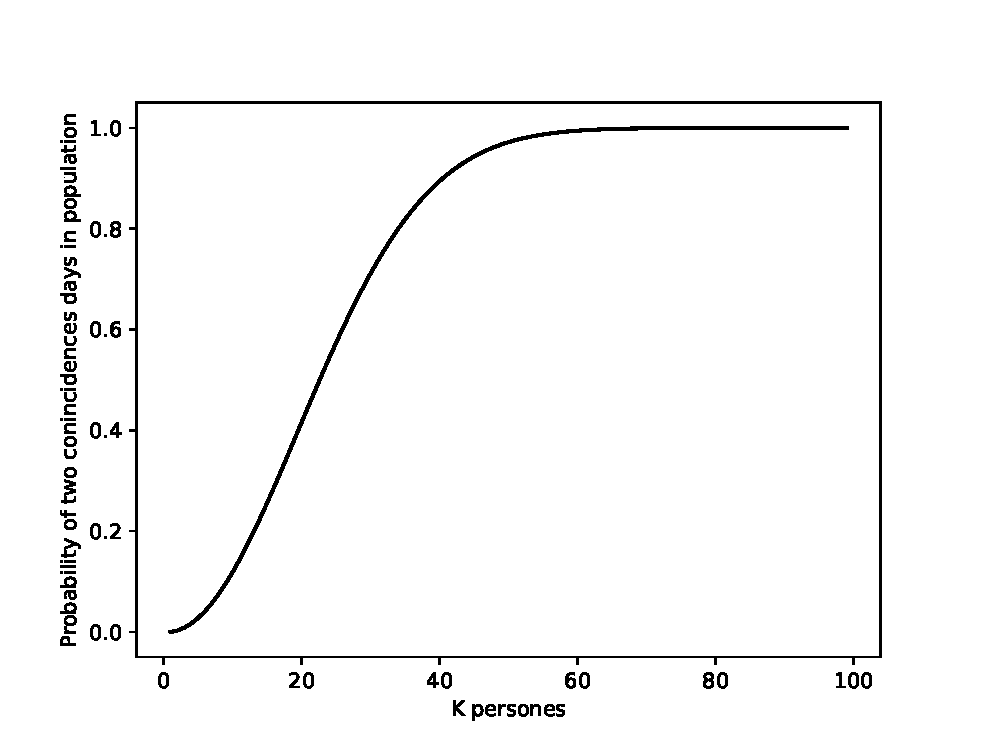
\includegraphics[scale=0.55]{paradox.eps}}
\caption{Birthday paradox with 360 days}
\label{fig}
\end{figure}
\end{frame}





\begin{frame}{of 1-1, 2-2,... k-k}
The problem consist in estimate the total number of combinations of genes, therefore:

\begin{equation}
\sum_{i=1}^{n} \binom{n}{i}
\end{equation}
however implementing this  require $n$ computations of \textit{fact} or \textit{factl} defined previously, notice that $\sum_{i=0}^{n} \binom{n}{i} & = 1 + \sum_{k=1}^{n}\binom{n}{k} $.

\begin{equation}
\begin{split}		
    (x+y)^{n} &= 1 + \sum_{k=1}^{n} \binom{n}{k}x^{n-k}y^{k}
\end{split}
\end{equation}

if we suppose that $x$ and $y$, both are equal to one, then.
\begin{equation}\label{end}
2^{n}-1 = \sum_{i=1}^{n}\binom{n}{k}
\end{equation}
 \end{frame}





\begin{frame}[fragile]{Geometric Distribution}
Model the number of failures that we need to carry out until reach a success. For instance, the number of trials with vaccination needed to reach that the vacumn be useful.

\begin{equation}
P(X=x) = (1-p)^{x-1}p
\end{equation}

How many test we must carry out until the first infected patient will be selected.

\begin{lstlisting}
def geometric(p,x):
  if p>1 or p<0:
    print('P must be a probability')
  else:
    return ((1-p)**x)*p
\end{lstlisting}
\end{frame}



\begin{frame}[fragile]{list comprehension}
Composed of expression, if - clauses, and loops.
\begin{lstlisting}
[exp for i in iterable]
odds = [["par",i] if i%2==0 else ["impar",i] for i in range(1,11)]
print(odds)
\end{lstlisting}
\end{frame}

\begin{frame}[fragile]{Geometric Comparation}
\begin{lstlisting}
def geometric(p,x):
  if p>1 or p<0:
    print('P must be a probability')
  else:one
    return ((1-p)**x)*p
p = [ 3, 12, 24, 33]
k=22
for x in p:
  exec(f"p_{x} = [geometric({x/100},i) for i in range(k)]")
  exec(f"plt.plot(np.arange(k),p_{x})")
\end{lstlisting}
\end{frame}






\begin{frame}{Geometric CDF}{Cumulative Distribution Function}
The question it is $P(X>x)$.
\begin{equation}
CDF = 1-(1-p)^{k}
\end{equation}
\end{frame}




\begin{frame}{Memoryless}{Geometric Distribution}
Past events not affect future.
In the discrete time the geometric have this property and in continous the exponential distribution too. They are related?
\begin{theorem}
if $\mathbf{x} \sim geometric(p)$ then $P(X>x+y)$
\end{theorem}
\end{frame}

\begin{frame}{Negative Binomial distribution}

\end{frame}

\begin{frame}{Exponential- Geometric}{Exponential distribution}
$\mathbf{X} \sim exp(\lambda)$  count the time until a Bernoulli trial it is success, the trials are continous at a time of success $\lambda$

\end{frame}






\begin{frame}[fragile]{Dynamic code}
\begin{lstlisting}
for x in range(3):
	exec(f'var_{x}=x')
\end{lstlisting}
\end{frame}



\begin{frame}{Most popular libraries by statistical analysis}
\begin{itemize}
\item pandas
\item matplotlib
\item seaborn
\item os
\item statsmodels
\item scipy
\item numpy
\end{itemize}
\end{frame}


\begin{frame}[fragile]{let's star to programming}
you must type all that appear in the following theme, is very useful uses the script.
\begin{lstlisting}
import stats 
print(str(python for all))
\end{lstlisting}
\end{frame}



\begin{frame}[fragile]{STATISTICS library}
\textbf{statistics} library is integrated by default with  python installation it is useful to calculate, mean, median , mode and other statistics.
\begin{lstlisting}
import statistics
data=[1,2,3,4,5]
statistics.mean(data) #arithmetic mean
\end{lstlisting}
\end{frame}



\begin{frame}{statistics functions}
\begin{enumerate}
\item mean()
\item median()
\item mode()
\item stdev()
\item variance()
\end{enumerate}
\end{frame}


\begin{frame}[fragile]{Working directory}
the working directory is a path that indicates a python where input and otput files
for instance datasets, images or documents.  to know by default what is the current workign directory:
\begin{lstlisting}[fragile]
import os
print(os.getcwd())
dir=os.getcwd()
print(dir)
\end{lstlisting}
\end{frame}


\begin{frame}{Normality}
The normality is a concept derived of nature, that was mathematically encripted in some symbols:
\begin{equation}
f(x)= \frac{1}{\sigma \sqrt{2 \pi}}  e^{\frac{(x - \mu)^{2} }{ 2 \sigma^{2}}}
\end{equation}
\end{frame}



\begin{frame}[fragile]{Histogram}
what is the distribution of the variable regarding it self?
\begin{lstlisting}
plt.hist()
\end{lstlisting}
\end{frame}

\begin{frame}[fragile]{Visual relation between two variables}{scatter}
\begin{lstlisting}
plt.scatter(x,y,data="dataname")
\end{lstlisting}
\end{frame}




\begin{frame}[fragile]
we can compare strings.
indexing strings.
what it is the last position.
\begin{lstlisting}
element[-1],
\end{lstlisting}
Remember that in python index start in 0 and end in n-1.
\begin{lstlisting}
lista[beging:stop:step]
lista[::] = lista[0:len(s):1]
\end{lstlisting}
\end{frame}




\begin{frame}[fragile]{Break statement}
Sometimes we need stop the run or execution of a program, the \textbf{break} 
\begin{lstlisting}
k=222
limit = 19
ls=[]
for j in range(k):
    if j%2==0 :
        ls.append(j)
    if len(ls)>limit:
        break
print(ls)
print(len(ls))
\end{lstlisting}
The previous code will finish when the length of the list, reach a size greater than the limit. 
\end{frame}



\begin{frame}[fragile]{Continue statement}
In some cases we need avoid a condition, remaining in the cycle. 
\begin{lstlisting}
N=10
ls=[]
for l in range(N):
    if l==4 or l==6:
        continue
    elif l%2==0:
        ls.append(l)
print(ls)
\end{lstlisting}

\end{frame}


\begin{frame}[fragile]{Sorting}
\begin{lstlisting}
dat=[99,23,13,44,120,42,12]
new=[]
while len(dat)!=0 :
    k=dat[0]
    for j in dat:
        if k < j:
            k=j
    dat.remove(k)
    new.append(k)
print(new)
\end{lstlisting}
\end{frame}




\begin{frame}{Insights about recursion}
The process must be finish, in some cases, therefore we need establish a \textbf{base case}, that means the instance of the problem in wich the recursion must be over. 
\end{frame}





\begin{frame}[fragile]{Removing missing values}{Pandas}
This code will remove the missing values in all columns or rows. 
\begin{lstlisting}
import numpy as np
import pandas as pd 
import matplotlib.pyplot as plt
data = pd.DataFrame([[2,10,np.nan], [30,60,np.nan],[ np.nan,np.nan,np.nan]])
data.dropna(axis=0, how='all', inplace=True)
data.dropna(axis=1, how='all', inplace=True)
\end{lstlisting}
\end{frame}






\begin{frame}
good words:
unsavory: desagradable
rushed:precipitarse, apurado.
arguibly: posiblemente
amaze; asombrar.
advertise: anunciar

\end{frame}



\begin{frame}{Replacement -Order doest not matter}
\end{frame}






\begin{frame}{Poisson Distribution}
Poisson distribution is derived from  when the variable follow a binomial distribution with a  $n $ $\to$  $\infty $

In the limit case, the occurrence of  a only event is only guaranteed in the measure that the space is very small, for instance if the ocurrence of the events is simultaneous, you should not consider a Poisson distribution. $E(x)= np = \lambda$, thus ,$\frac{\lambda}{n}=p$  and according to FD of a $x \sim b(n,p)$

\begin{equation}
\begin{split}
PDF = &\frac{n!}{(n-k)!k!}(\frac{\lambda}{n})^{k} (1-\frac{\lambda}{n})^{n-k} \\
= &\frac{(n-k+1)!}{n^{k}k!} ( 1 - \frac{\lambda}{n})^{n}  ( 1 -\frac{\lambda}{n})^{-k}  \\
\end{split}
\end{equation}

$e=\lim_{x \to \infty} (1+\frac{1}{n})^n$we must use $t=\frac{n}{k}$,  and thus $ \frac{n+k}{n} = 1+\frac{k}{n}$
 $\lim_{n \to \infty} = \frac{e^{-k} \lambda^{k} }{k!}$ 
 
\begin{equation}
P(X=x)=\frac{e^{-x}\lambda^{x}}{x!}
\end{equation}
\end{frame}


\begin{frame}{Conjoint probability}
fooling;engañado.
disguise:
crew:tripulación,personal.
contestant:
spoil:arruinar, estropear.
try it out:
scathing
honing:afilado.
boggling:
wrecked: destrozado, arruinar.
bestowed: otorgado.
dumped:
claim: afirmar.
fully:
blunder:
conceals: oculta.
disregard: ignorar.
\end{frame}




\begin{frame}{inclusion-exclusion}

\end{frame}



\begin{frame}{Independece}
Independence not is equal not occurrence, the independence is related with the change of the probability that occur a event given that another occur.
\begin{equation}
P(A \cap B) = P(A)P(B)
\end{equation}
Tossing coins it is a bernoulli trial, and the occurrence of a event not affect the another event.
\end{frame}



\begin{frame}{Contingency table}
\begin{table}[]
\begin{tabular}{lllccc}          &                               &                                & \multicolumn{3}{c}{\textbf{Diagnose}}                                               \\ \cline{4-6} 
          &                               &                                & \multicolumn{1}{l}{Disease} & \multicolumn{1}{l}{} & \multicolumn{1}{l}{No-Disease} \\ \cline{4-6} 
          & \multicolumn{1}{l|}{}         & \multicolumn{1}{l|}{Smoke}     & a                           &                      & b                              \\
\multicolumn{2}{l|}{\textbf{Risk Factor}} & \multicolumn{1}{l|}{}          &                             &                      &                                \\
          & \multicolumn{1}{l|}{}         & \multicolumn{1}{l|}{Not Smoke} & c                           &                      & d                              \\
          &                               &                                & \multicolumn{1}{l}{}        & \multicolumn{1}{l}{} & \multicolumn{1}{l}{}          
\end{tabular}
\end{table}
What it is $P(Disase \mid Smoke) = \frac{a}{a+b}$ 
note that marginal distribution.  Note that $P(Disease \cap Smoke) = \frac{a}{(a+b+c+d)}$. Also note that $P(Smoke)= \frac{a+b}{(a+b+c+d)}$. Note the result of divide the last two probabilities.
\end{frame}




\begin{frame}{Conditional Probability}

The probability of event given a "information".\emph{Probability of $A$ occur given $B$ occurs. }

\begin{equation}
P(A \mid B) = \frac{P(A \cap B)}{P(B)}
\end{equation}

Note that $P(A \cap B)$ it is equal to $P(B \cap A)$.

\begin{equation}
P(A \mid B)P(B) = P(B \mid A)P(A)
\end{equation}
\end{frame}


\begin{frame}{Bayes theorem}
Notice that not is same: 
\emph{The probability that occur A given B, that occur B given A.} However we can compute one of the another.
\begin{equation}
P(A \mid B) = \frac{P(A) P(B \mid A)}{P(B)}
\end{equation}
\end{frame}



\begin{frame}{Bowls problems}
Derive the following problem.
\end{frame}




\begin{frame}{Law of total probability}
The sample space defined as $\Omega$ 
if we split omega in $\omega$ $k$ subsets in order that each $subset$ no overlap with others.
$\bigcup_{i=1}^{k} \omega_{i} = \Omega $ y $
\bigcap_{i=1}^{k} \omega_{i} = \emptyset
$
For instance the sample space defined as $ \Omega= \lbrace a ,b,c,d,e,f\rbrace$
$\omega_{1}=\lbrace a,f \rbrace$  $\omega_{2}=\lbrace b,c,d \rbrace  $ $ \omega_{3}=\lbrace e \rbrace $.
\end{frame}


\begin{frame}{Split $\Omega$}
\begin{figure}

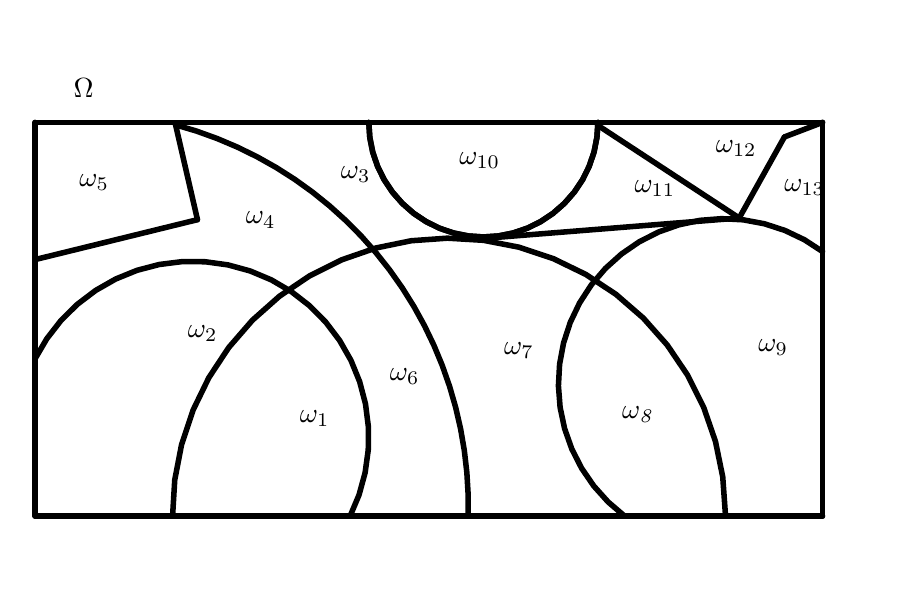
\begin{tikzpicture}[line cap=round,line join=round,>=triangle 45,x=1cm,y=1cm]
\clip(-12.095168341119958,-1.8253174810990838) rectangle (-1.4053738900064559,5.203119715631769);
\draw [line width=2pt] (-12,4)-- (-6,4);
\draw [line width=2pt] (-12,4)-- (-12,-1);
\draw [line width=2pt] (-6,4)-- (-2,4);
\draw [line width=2pt] (-2,4)-- (-2,-1);
\draw [line width=2pt] (-12,-1)-- (-2,-1);
\draw [shift={(-10,0)},line width=2pt]  plot[domain=-0.46364760900080615:2.677945044588987,variable=\t]({1*2.23606797749979*cos(\t r)+0*2.23606797749979*sin(\t r)},{0*2.23606797749979*cos(\t r)+1*2.23606797749979*sin(\t r)});
\draw [shift={(-11.52,-0.88)},line width=2pt]  plot[domain=-0.023899830887098794:1.308676485529425,variable=\t]({1*5.021434058115271*cos(\t r)+0*5.021434058115271*sin(\t r)},{0*5.021434058115271*cos(\t r)+1*5.021434058115271*sin(\t r)});
\draw [shift={(-6.744941662832751,-0.98)},line width=2pt]  plot[domain=0.005697944032979157:3.147290597622772,variable=\t]({1*3.510056979594493*cos(\t r)+0*3.510056979594493*sin(\t r)},{0*3.510056979594493*cos(\t r)+1*3.510056979594493*sin(\t r)});
\draw [shift={(-3.2567368200552362,0.679872248814668)},line width=2pt]  plot[domain=0.9285030181026769:4.07009567169247,variable=\t]({1*2.0979414213033207*cos(\t r)+0*2.0979414213033207*sin(\t r)},{0*2.0979414213033207*cos(\t r)+1*2.0979414213033207*sin(\t r)});
\draw [shift={(-6.30779124440237,4)},line width=2pt]  plot[domain=3.141592653589793:6.283185307179586,variable=\t]({1*1.454939050215934*cos(\t r)+0*1.454939050215934*sin(\t r)},{0*1.454939050215934*cos(\t r)+1*1.454939050215934*sin(\t r)});
\draw [shift={(-6.30779124440237,4)},line width=2pt]  plot[domain=3.141592653589793:6.283185307179586,variable=\t]({1*1.454939050215934*cos(\t r)+0*1.454939050215934*sin(\t r)},{0*1.454939050215934*cos(\t r)+1*1.454939050215934*sin(\t r)});
\draw [line width=2pt] (-12,2.258002259588651)-- (-9.93853929509727,2.764562471815984);
\draw [line width=2pt] (-9.93853929509727,2.764562471815984)-- (-10.218480465012375,3.9776408747814385);
\draw (-11.636643227019698,4.676158017337441) node[anchor=north west] {$\Omega$};
\draw [line width=2pt] (-2,4)-- (-2.4843671441318684,3.8153244435494);
\draw [line width=2pt] (-2.4843671441318684,3.8153244435494)-- (-3.0587180577304687,2.7858275229481317);
\draw [line width=2pt] (-4.851660403825104,3.9608761613021164)-- (-3.0587180577304687,2.7858275229481317);
\draw [line width=2pt] (-6.4346664749495215,2.516316534266319)-- (-3.0587180577304687,2.7858275229481317);
\draw (-8.76230669086882,0.46730808940221685) node[anchor=north west] {$\omega_{1}$};
\draw (-6.736583798724393,3.7454204722981066) node[anchor=north west] {$\omega_{10}$};
\draw (-7.619415734827877,0.9942697876965457) node[anchor=north west] {$\omega_{6}$};
\draw (-6.168560149913624,1.3296090502474822) node[anchor=north west] {$\omega_{7}$};
\draw (-2.9383533759535907,1.3638273423445166) node[anchor=north west] {$\omega_{9}$};
\draw (-4.669798956063524,0.515213698338065) node[anchor=north west] {$\mathit{\omega_{8}}$};
\draw (-11.561362984406223,3.4648304771024248) node[anchor=north west] {$\omega_{5}$};
\draw (-8.2421886509939,3.560641694974121) node[anchor=north west] {$\omega_{3}$};
\draw (-4.512394812417166,3.3895502344889494) node[anchor=north west] {$\omega_{11}$};
\draw (-10.185787642105446,1.548606119668502) node[anchor=north west] {$\omega_{2}$};
\draw (-3.479002391086732,3.8959809575250577) node[anchor=north west] {$\omega_{12}$};
\draw (-2.6098577718220617,3.4032375513277633) node[anchor=north west] {$\omega_{13}$};
\draw (-9.446672532809506,2.985774387743944) node[anchor=north west] {$\omega_{4}$};
\end{tikzpicture}
\end{figure}
\end{frame}

\begin{frame}{$P(A)$}{total law probability}
We need remember by set theory that a event $A$ could be rewrite as $A  = (A \cap B) \cup (A \cap C)$. 
if $(B \cup C ) = \Omega $
for this case we can rewrite 
\begin{equation}
\begin{split}
A &= (A \cap \omega_{1}) \cup ( A \cap \omega_{2})...(A \cap \omega_{k})
\\
P(A)&= P(A \cap \omega_{1}) + ... + P(A \cap \omega_{k})
\\
P(A) &= P( A \mid \omega_{1} )P(\omega_{1}) + P(A \mid \omega_{2}  )P(\omega_{2}) +...+  P( A \mid \omega_{k})P(\omega_{k})
\end{split}
\end{equation}

note that  by total law $P(A)$ 
\end{frame}


\begin{frame}{Monty Hall simulation}
\begin{block}

This problem is so not intuitive that generated controversy in the academic community. 
\end{block}

There are three closed doors,  and you must select one to win  a car,  behind the doors, there is a car, and behind the other two there are goats. After select the door, another door with a goat it is showed to you, then you can change your first election,  the main problem is if you must remain in the selected door or change?

Notice that the initial probability of win the car is the 1/3.
\end{frame}



\begin{frame}{Monty Hall simulation}{}
\begin{figure}[htbp]
\centerline{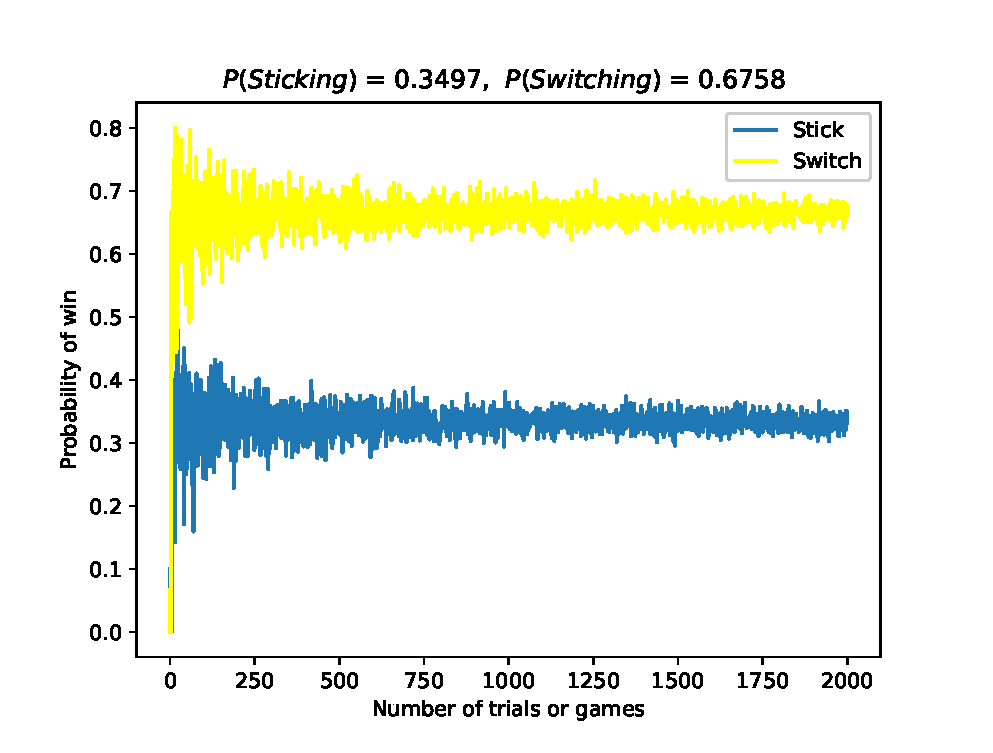
\includegraphics[scale=0.66]{./graphs/Monty.eps}}
\end{figure}
\end{frame}





\begin{frame}[fragile]{Monty Hall problem}{Python code}
\begin{lstlisting}
def monty_game():
  doors=[1,2,3]
  doors_variable = doors.copy()
  winner = random.randint(1,3)
  select_one = random.randint(1,3)
  values = [winner,select_one]
  switch = list( set(doors) - set(values))
  select_two = random.randint(switch[0], switch[-1])
  s1,s2 = 0,0
  if winner == select_one:
    s1 += 1
  else:
    s2 +=1
  return [s1,s2]
\end{lstlisting}
\end{frame}


\begin{frame}[fragile]{Monty Hall problem}{Python code}
\begin{lstlisting}
trials=2000
s1_=[]
s2_=[]
for n in range(1,trials):
  prob_s1 = sum([monty_game()[0] for _ in range(1,n)])/n
  s1_.append(prob_s1)
  prob_s2 = sum([monty_game()[1] for _ in range(1,n)])/n
  s2_.append(prob_s2)
plt.plot(np.arange(1,trials),s1_, label='Stick')
plt.plot(np.arange(1,trials),s2_, label='Switch',color='yellow')
plt.title('$P(switching)$ = {:.4},  $P(sticking)$ = {:.4} '.format(prob_s1,prob_s2))
\end{lstlisting}
\end{frame}



\begin{frame}{Monty Hall}{Bayesian solution}
The event $D_{i}$ the $i$ winner door and  $M_{j}$ monty open $j$ door, for $i,j=1,2,3$.

\begin{equation}
P(D_{i} \mid M_{j}) = \frac{P(M_{j} \mid D_{i})P(D_{i})}{P(M_{j})}
\end{equation}

you select the first door  and monty the second, therefore the question  is $P(D_{3} \mid M_{2})$.
Notice that $ P(M_{2}) = \sum_{i=1}^{3} P(M_{2} \mid D_{i}) $.  
given the rules of game, 
$P(M_{2} \mid D_{2}) = 0$, and 
$P(M_{2} \mid D_{3}) = 1$, if monty could select random in two choices $P(M_{2} \mid C_{1})=1/2$ and finally, switch strategy have a probability of 2/3.
\end{frame}







\begin{frame}{Buffon Needled}
\begin{columns}

\column{0.5\textwidth}
Here we have a column


\column{0.5\textwidth}

we have another column


\end{columns}

\end{frame}


\begin{frame}[fragile]{$\pi$ Number}

\begin{columns}


\column{0.5 \textwidth}
\begin{lstlisting}
import numpy as np
import matplotlib.pyplot as plt
dots = 5000
c1,c2=-1,1
x = np.random.uniform(c1,c2, size=dots)
y = np.random.uniform(c1,c2, size=dots)
coordenates_circle = (x**2)+(y**2) < 1
circle_y=y[coordenates_circle]
circle_x=x[coordenates_circle]
pi = 4*sum(coordenates_circle) / dots
plt.scatter(x,y, color='yellow')
plt.scatter(circle_x,circle_y)
\end{lstlisting}

\column{0.5 \textwidth}
What is the probability of a drop lands in the circle?
\begin{equation}
P(hit) = \frac{\pi r^{2}}{4r^{2}}
\end{equation}
\begin{figure}
\centerline{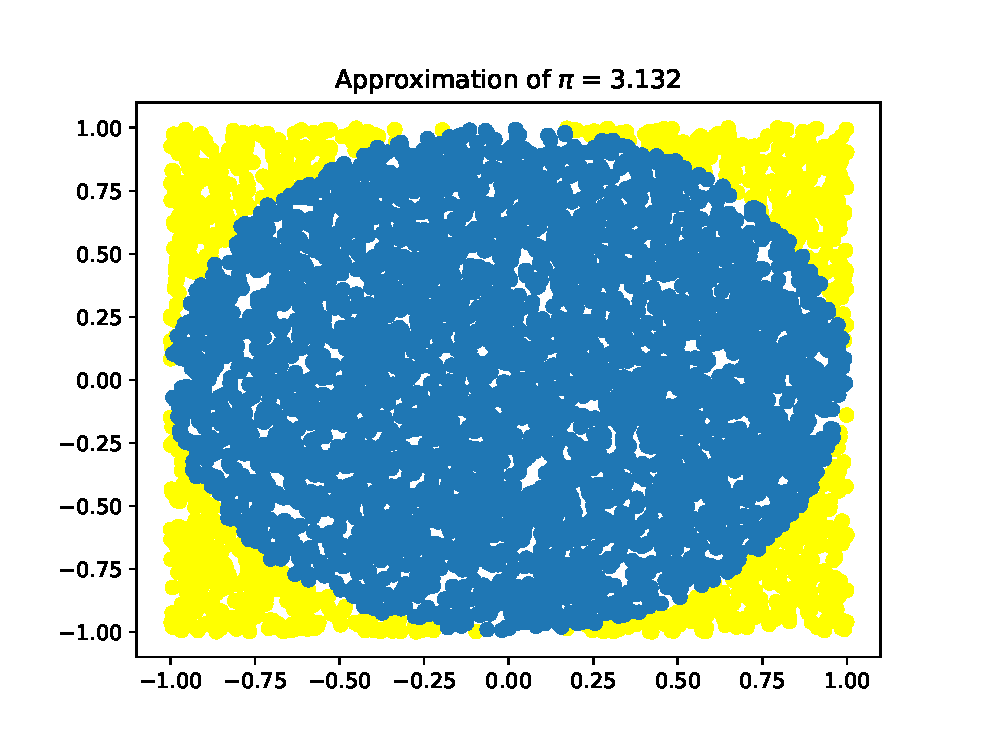
\includegraphics[scale=0.4]{./graphs/PiOne.eps}}
\label{fig}
\end{figure}
\end{columns}
\end{frame}



\begin{frame}{Needles}
Proposed by and resolved by the naturalist. take in mind the 
\begin{figure}
\definecolor{ududff}{rgb}{0.30196078431372547,0.30196078431372547,1}
\begin{tikzpicture}[line cap=round,line join=round,>=triangle 45,x=1cm,y=1cm]
\clip(-12.564766534876606,0.22190923729896378) rectangle (-2.0940558311248365,7.241112822647047);
\draw [line width=2pt] (-12,6)-- (-12,1);
\draw [line width=2pt] (-10,6)-- (-10,1);
\draw [line width=2pt] (-8,6)-- (-8,1);
\draw [line width=2pt] (-4,6)-- (-4,1);
\draw [line width=2pt] (-6,6)-- (-6,1);
\draw [line width=2pt] (-12,6)-- (-4,6);
\draw [line width=2pt] (-12,1)-- (-4,1);
\draw [line width=2pt] (-10,4)-- (-9,4);
\draw [line width=2pt] (-8.296193565998552,2.4731031062869198)-- (-7.5965657346611755,3.0081126243684424);
\draw [line width=2pt] (-10.381358867239362,2.418230335201635)-- (-9.681731035901985,1.938093588205397);
\draw [line width=2pt] (-4.468817782799958,3.3922220219654338)-- (-5.2096001924513,2.8572125038839107);
\draw [line width=2pt] (-6.965528867180401,4.571986600299049)-- (-6.1012827225871735,4.242749973787341);
\draw [line width=2pt] (-7.1164289876649365,1.4579568412091586)-- (-6.238464650300384,1.1424384074687728);
\begin{scriptsize}
\draw [fill=ududff] (-9,4) circle (2.5pt);
\draw [fill=ududff] (-8.296193565998552,2.4731031062869198) circle (2.5pt);
\draw [fill=ududff] (-10.381358867239362,2.418230335201635) circle (2.5pt);
\draw [fill=ududff] (-4.468817782799958,3.3922220219654338) circle (2.5pt);
\draw [fill=ududff] (-6.965528867180401,4.571986600299049) circle (2.5pt);
\draw [fill=ududff] (-6.238464650300384,1.1424384074687728) circle (2.5pt);
\end{scriptsize}
\end{tikzpicture}
\end{figure}
\end{frame}




\begin{frame}[fragile]{Uniform distribution}
\begin{columns}
\column{0.5 \textwidth}
$\mathbf{x} \sim U(a,b)$ in the interval$(a,b)$.
\begin{equation}
f(x) = \frac{1}{b-a}
\end{equation}
the function is defined in the open interval  $a<x<b$.
Remember that:
\begin{equation}
F(x) = \int_{- \infty}^{x}f(u)du
\end{equation}

\column{0.5\textwidth}
\begin{lstlisting}
import numpy as np
np.random.uniform(a,b ,size=(k,p)) # [)

#Draw k list with p elements with numbers [a,b)
\end{lstlisting}
Choose a point in the interval (a,b), you can calculate what it is the probability that a point is in (c,d) 
\end{columns}
\end{frame}



\begin{frame}{Deck of cards}{52 standard}
There are 4 'types'(suits), clubs, diamonds, 

\end{frame}


\begin{frame}{Gamblers ruin}

\end{frame}







\begin{frame}{Topics to research}
\begin{itemize}
\item Conditional indepedence
\item Panzer ruin
\item vander
\end{itemize}
\end{frame}


\begin{frame}[fragile]{Matrix}
\begin{lstlisting}
matrix = [[1,2,3],[10,11,12],[18,19,29]]
\end{lstlisting}

\end{frame}




\begin{frame}[fragile]{Matrix}{Sum}
\begin{lstlisting}
def sum_matrix(matA, matB):
  rows = len(matA)
  column =len(matA[0])
  if len(matA) != len(matB):
    raise Exception('Dont have the same number of rows')
  sum_mat = []
  for i in range(0,rows):
    row =[]
    for j in range(0,column):
      row.append(matA[i][j]+matB[i][j])
    sum_mat.append(row)
  return sum_mat
\end{lstlisting}
\end{frame}




\begin{frame}[fragile]{Matrix tranpose}

\begin{lstlisting}

def transpose(matx):
  transpose_mat=[]
  for h in range(0,len(matx[0])):
    row =[]
    for j in matx:
      row.append(j[h])
    transpose_mat.append(row)
  return transpose_mat
\end{lstlisting}
\end{frame}




\begin{frame}[fragile]{identity}
\begin{lstlisting}
def nrow(size,row_n):
    row = []
    for j in range(0,size):
      if j == row_n-1:
        row.append(1)
      else:
        row.append(0)
    return row
\end{lstlisting}
\end{frame}

\begin{frame}[fragile]{identity}
\begin{lstlisting}
def indentity(matrix):     # we also could take min ( column, row) and return a square of these size
  # check if square
  check = len(matrix)
  for j in matrix:
    if len(j)!= check:
      raise Exception("Not is a square MATRIX")
  mat=[]
  for j in range(1,check+1):
    mat.append(nrow(check,j))
  return mat
\end{lstlisting}
\end{frame}



\begin{frame}[fragile]{inner product}
\begin{lstlisting}
def inner(vectorA,vectorB):
  if len(vectorA) != len(vectorB):
    raise Exception('overcome dimensionality')
  column = len(vectorA)
  addedVector = []
  for j in range(0,column):
    if type(vectorB[j])==list:
      addedVector.append(vectorA[j] * vectorB[j][0])
    if type(vectorB[j])!=list:
      addedVector.append(vectorA[j] * vectorB[j])
  return sum(addedVector)
\end{lstlisting}
\end{frame}


\begin{frame}[fragile]{ Product}
\begin{lstlisting}
def prod(matA, matB):
 row = len(matA)
 col = len(transpose(matB))
 resultado = []
 for j in range(0,row):
   row =[]
   for i in range(0,col):
    row.append(inner(matA[j],transpose(matB)[i]))
   resultado.append(row)
 return resultado
\end{lstlisting}
\end{frame}



\begin{frame}{Numpy}
What is numpy and why it is important?
numpy is a open source project, that allow us work with arrays.

np.arrays are most fast than built-in lists.

some functions of numpy are written in C or C++.


\end{frame}


\begin{frame}[fragile]{Inner(dot) product}
\begin{equation}
\begin{align*}
\vec{u}.\vec{v} &= \sum u_{i} v_{i} \\
\vec{u}.\vec{u} &= \frac{n(n+1)(2n+1)}{6}
\end{align*}
\end{equation}
\begin{lstlisting}
a = np.array([1,2,3,4])
b = np.array([1,3,4,4))
np.dot(a,b)

def sum_square(number):
  return  number * (number+1) * (2*number +1 ) / 6
sum_square(6)
\end{lstlisting}
\end{frame}


\begin{frame}[fragile]{Matrix multiplication}{@}
When the arrays are of 1-D then uses$np.dot()$ otherwise, 2-D arrays uses $np.matmult()$ or $@$.

\begin{equation}
\[
A B = 
\begin{pmatrix}
1 & 2  & 3 \\
1 & 5 & 2 \\
4 & 2 & 0 
\end{pmatrix}
\begin{pmatrix}
1 & 0 \\
0 & 1 \\
1 & 0
\end{pmatrix}
=
\begin{pmatrix}
4 & 5 \\
3 & 7 \\
4 & 2
\end{pmatrix}

\end{equation}


\begin{lstlisting}
A = np.array([[1,2,3], [1,5,2], [4,2,0]])
B = np.array([[1,0],[0,1],[1,0]])
A @ B
np.matmul(A,B)
\end{lstlisting}

\end{frame}



\begin{frame}[fragile]{Numpy}{other functions}
\begin{lstlisting}
np.zeros((rows,columns)) #Return a array of zeros.
np.transpose(array) # Return the transpose matrix.
np.ones_like(array) # Return the array with the same size but filled with ones.
\end{lstlisting}
\end{frame}





\begin{frame}[fragile]{Switch}
\begin{lstlisting}
def funcion1():
  print('f1')
def funcion2():
  print('f2')
def funcion3():
  print('f3')
def switch(a):
  swithcer={1: funcion1, 
            2: funcion2,
            3: funcion3
  }
  return swithcer.get(a)()
switch(1)
\end{lstlisting}

\end{frame}



\begin{frame}{Duck typing}


\end{frame}



\begin{frame}{Dynamic typing}
python remember only the last assigment.
The last assignment to a 'variable' is the last value.

\end{frame}

\begin{frame}[fragile]{Type hints}
We said previously that is important in object oriented programming, to know, what type of object will be returned by a function, this allow us read more easily the code.

To write better code
\begin{lstlisting}
def factorial(n:int) -> int:
statements..
\end{lstlisting}
This is a way of write better code, but take time.
\end{frame}



\begin{frame}[fragile]{Type hints}

\begin{lstlisting}
def factorial(n:int) -> int:
acum: int = n 
for x in range(1,n):
	acum: int = acum + x
return acum

\end{lstlisting}
This is a way of write better code, but take time.
\end{frame}


\begin{frame}[fragile]
To see documentation about type hints.
\begin{lstlisting}
factorial.__annotations__
\end{lstlisting}
\end{frame}



\begin{frame}[fragile]
types
\begin{lstlisting}
int, float,str, NoneType
\end{lstlisting}
\end{frame}





\begin{frame}{Unicode}
is a standard to codify characters, 
in python the function ord() return its code.
ASCII values..
\end{frame}






\begin{frame}[fragile]{Prime number}
\begin{lstlisting}
def prime(k):
  i =1
  flag = False
  while flag==False and i<k-1:
    i = i+1
    if k%i==0:
      flag=True
  if flag==True:
    return 'no primo'
  else:
    return 'primo'
prime(7)
\end{lstlisting}
\end{frame}


\begin{frame}[fragile]{Split own implementation}
\begin{lstlisting}
def split(text, char):
  joint, result = '', []
  for letter in text:
    if letter == char:
      result.append(joint)
      joint = ''
    else:
      joint = joint + letter
  return result
\end{lstlisting}
\end{frame}






\begin{frame}[fragile]{Ceaser code criptography}
\begin{lstlisting}
def cripto(text,constant):
  result = ''
  for letter in text:
    letter_coded = str(ord(letter)+ constant) + '-'
    result  = result + letter_coded 
  result = result[0:-1]
  return result

def decifre(text,constant):
  result  = ''
  for code in text:
    decode = chr(int(code)-constant)
    result = result + decode
  return result
\end{lstlisting}
\end{frame}



\begin{frame}[fragile]{Dynamic vs static typing}
we said that the language follow a static programming style if the variables must be defined in compilation time. Otherwise, dynamic programming define variables in execution time.

\begin{verbatim}
int c = 10
\end{verbatim}

\end{frame}

\begin{frame}[fragile]
strong and weak typing:
python have a strong typing for instance
\begin{lstlisting}
a = 10
b = '1'
print(a+b)
\end{lstlisting}
this will araise a error, in a weak language one variable cast to compatible type for instance to concatenate, '101'.

Python allow us a static system with type hints, for instance;
\begin{lstlisting}
var: float = 10.1
\end{lstlisting}
\end{frame}


\begin{frame}[fragile]{mypy}
spite of the ability of python to be explicit definition of type, not guaranteed that the parser arise a error if the variable change of type in execution time.
we can uses mypy to check the consistency.

if we want a variable that change in the execution then we could define as:
\begin{lstlisting}
from typing import Any
var: Any = 10
\end{lstlisting}
Then mypy not raises a error.
\end{frame}

\begin{frame}[fragile]{Delete functions}
\begin{lstlisting}
del function_Name
\end{lstlisting}
\end{frame}


\begin{frame}[fragile]{Modules and packages}
\textbf{import} it is a keyword.
the package will be loaded, if there is in path, python search the module in the current directory, and after in PYTHONPATH.

\begin{lstlisting}
sys.path # Directories to load modules

\end{lstlisting}
\end{frame}



\begin{frame}[fragile]{Namespace}
Could exist two or more variables with the same name, living in different namespace. The scope of a variable play a key role: \textbf{global} variable could be invoked inside or outside of a function, otherwise a \textbf{local} variable only could be invoked inside the function(this imply that the variable was defined in the same function).
\end{frame}


\begin{frame}{local and global scope}
\textbf{global} refer to the ability to access in all program, and \textbf{local} only for parts of code.
When you define a variable, or assign a value inside a function, its scope is local.
If two variables have the same name, local variable override the global.

\end{frame}

\begin{frame}[fragile]{Namespace and scope}
variables are identifiers mapping to the objects stored in memory, a dictionary of variables names is called \textbf{Namespace}. Each function has its corresponding namespace.

\end{frame}





\begin{frame}[fragile]{Namespace and scope}
In each invocation of a function, it was created a scope, and this is destroyed when appear return.
\begin{lstlisting}
def function(x):
	result = ...
def function_(x):
	result = ...
\end{lstlisting}
Notice that \textbf{result} do not clash or rise a error, due both variables are defined in local scope. this means that is not allowed be invoked from another side of its own scope.
\end{frame}




\begin{frame}{LEGB rule}{Local,Enclosing,Global, Built-in}

\textbf{paradigm of Scope} this mechanism avoid collision by names,
python names could came from: Assignments, import , def and Class.

\begin{itemize}
\item Local scope: python functions or lambda expressions
\item Enclosing or nolocal: Nested functions
\item Global: related to the module, visible in all program.
\item Built-in: have keywords, functions, exceptions, that are built in.
\end{itemize}
This rule is a hierarchical structure for searching or call a variable.

\end{frame}



\begin{frame}[fragile]{Symbol table}
Is a data structure that contain information about; Methods,classes, variables, and so on of a program.
there are global and local tables:
\begin{lstlisting}
globals()
locals()
\end{lstlisting}
When you import a module this not is loaded automatically in symbol table
only the module name, therefore is needed access by the module name; for instance \textbf{np.float()} It
is important to know that each module have its own symbol table.
\end{frame}





\begin{frame}[fragile]{dir}
the \textbf{dir()} function tell us that things are inside of a package.
\begin{lstlisting}
dir(module_name)
\end{lstlisting}
could be useful to remember methods and attribute inside a package.
\end{frame}


\begin{frame}[fragile]{\_\_main\_\_}
Sometimes you write a module to be imported and its behavior must be change regarding if itself is the main program o will be part of another program.
\begin{lstlisting}
if __name__=='main':
	print('the main program never will be imported')
	
else:
	print('was loaded and not be a main program')
\end{lstlisting}
save the last snippet as \textbf{two.py}

\begin{lstlisting}
import two
print('this is main and was be executed form shell')	
\end{lstlisting}
save as \textbf{one.py} and execute in shell
\begin{verbatim}
python3 
\end{verbatim}
\end{frame}





\end{document}